本章では Icarus Verilog/NC-Verilog/VCS での論理シュミレーションの実行時間と
ArchHDL での実行時間を比較し,評価する.

Icarus Verilog/ArchHDL の実行環境は OS が Ubuntu12.04,カーネルが 64ビットの
Linux 3.2.0-39-generic, CPU は
Intel Core i7-3770K CPU @ 3.50GHz,メモリーは
$16\,\mathrm{GB}$ である.

NC-Verilog/VCS の実行環境は OS が CentOS5.9,カーネルが 64ビットの
Linux 2.6.18-348.4.1.el5, CPU は
hogehoge,メモリーは
$16\,\mathrm{GB}$ である.


## 並列化によらない高速化の評価

カウンター回路を $n$ 回試行するもの.

$n$ 個のカウンター回路を実行するもの.

\begin{figure}[t]
 \centering
 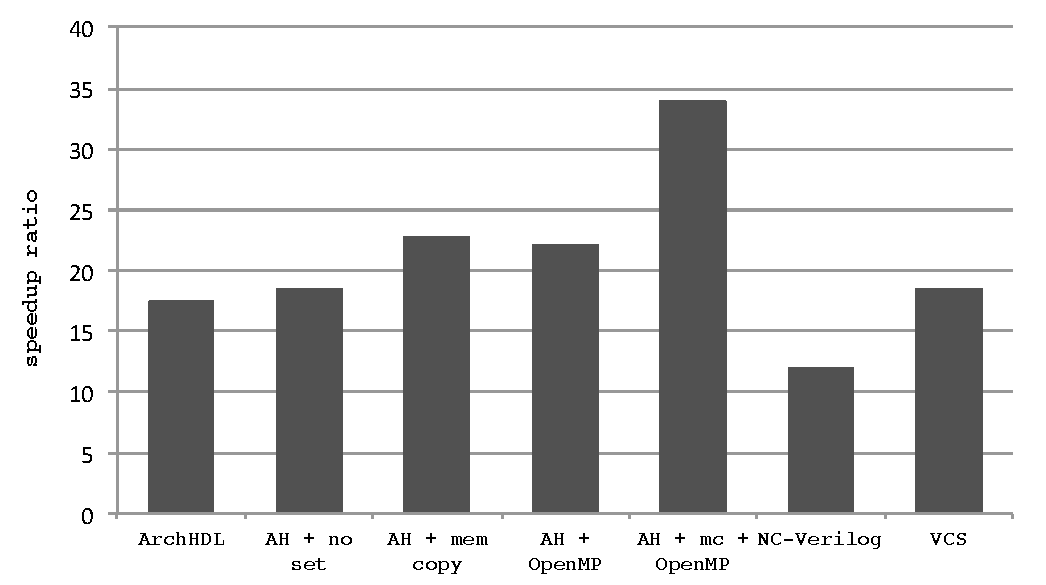
\includegraphics[clip,width=(\textwidth-\columnsep)/2]{stencil}
 \caption{ステンシル計算回路の Icarus Verilog と比較した実行時間の速度向上比}
 \label{fig:stencil}
\end{figure}

\figref{fig:stencil} はステンシル計算回路での実行結果である.

縦軸は Icarus Verilog と比較したそれぞれの速度向上比である.

NC-Verilog は ArchHDL より高速でない.VCS は ArchHDL の v1.0 と v1.1 より高速であるが, v2.0 よりは高速でない.また並列化を行ったものより高速でない.





XORSHIFT による乱数生成器.




ルータ





## 並列化による高速化の評価

\ref{ss:parallel} 節で述べたように `Singleton` クラスの `Exec()`
メソッドを OpemMP で並列化する.今回はスレッド数は 8 個で並列化を行う.







## 高速化の解析







